\documentclass{report}

% Packages
\usepackage[utf8]{inputenc}
\usepackage{graphicx}
\usepackage{float}
\usepackage{listings}
\usepackage{hyperref}
\usepackage[square,sort,comma,numbers]{natbib}
\usepackage{url}
\usepackage[strings]{underscore}

% Colores de los bloques de código
% All in preamble:

\usepackage{listings}
\usepackage{courier}
\usepackage{color}

\definecolor{codegreen}{rgb}{0,0.6,0}
\definecolor{codegray}{rgb}{0.5,0.5,0.5}
\definecolor{codepurple}{rgb}{0.58,0,0.82}
\definecolor{backcolour}{rgb}{0.95,0.95,0.92}

\lstdefinestyle{mystyle}{
    backgroundcolor=\color{backcolour},   
    commentstyle=\color{codegreen},
    keywordstyle=\color{magenta},
    numberstyle=\tiny\color{codegray},
    stringstyle=\color{codepurple},
    basicstyle=\ttfamily\footnotesize,
    breakatwhitespace=false,         
    breaklines=true,                 
    captionpos=b,                    
    keepspaces=true,                 
    numbers=left,                    
    numbersep=5pt,                  
    showspaces=false,                
    showstringspaces=false,
    showtabs=false,                  
    tabsize=2
}

\lstset{style=mystyle}


\hypersetup{
    colorlinks=true,
    linkcolor=blue,
    filecolor=magenta,      
    urlcolor=cyan,
    pdftitle={Overleaf Example},
    pdfpagemode=FullScreen,
}

\begin{document}

\begin{titlepage}
    \begin{center}
        \vspace*{1cm}
 
        \Large\textbf{Análisis aerolínea}
 
        \vspace{0.5cm}
        Práctica obligatoria 
             
        \vspace{1.5cm}
 
        \textbf{Antonio Cabrera}
 
        \vfill
             
        Trabajo para el doble grado de\\
        Ingeniería del Software y Matemática Computacional\\
             
        \vspace{0.8cm}
      
        
\includegraphics[width=0.4\textwidth]{figures/logo.png}
             
        Asignatura de procesamiento de datos\\
        U-tad\\
        España\\
        Mayo 2024
             
    \end{center}
 \end{titlepage}

\tableofcontents
\listoffigures

\chapter{Preparación del entorno de la máquina virtual}

Partiremos de la máquina virtual proporcionada por el profesor, la cual tiene instalado el sistema operativo Ubuntu 22.04.3 LTS.

\section{Preparación de Cassandra}

Primero instalaremos Cassandra, para ello primero actualizaremos el sistema operativo. El comando \texttt{sudo apt update} actualiza la lista de paquetes disponibles y sus versiones, mientras que el comando \texttt{sudo apt upgrade} instala las actualizaciones disponibles.

\begin{lstlisting}[language=bash]
sudo apt update && sudo apt upgrade
\end{lstlisting}

\begin{figure}[H]
    \centering
    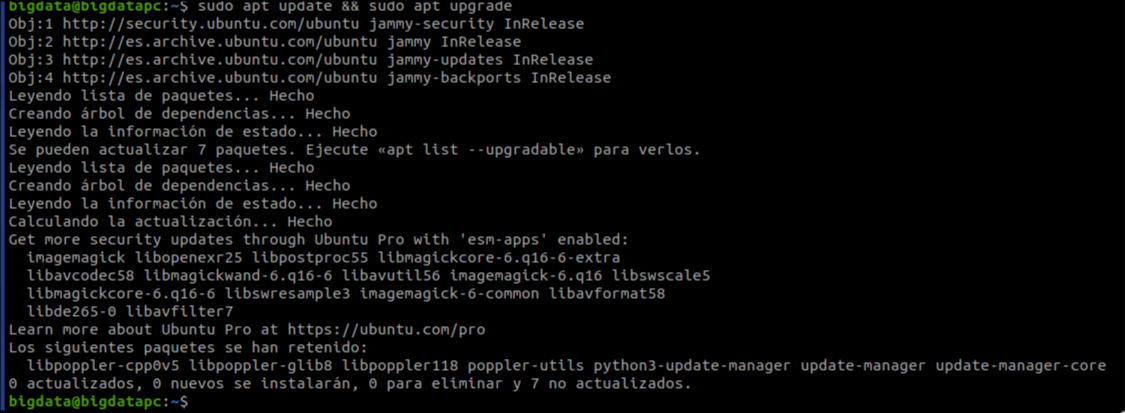
\includegraphics[width=0.8\textwidth]{figures/1.png}
    \caption{Actualización del sistema operativo}
\end{figure}

Ahora instalaremos Python 2, ya que Cassandra requiere esta versión de Python. Para ello, ejecutamos el siguiente comando:

\begin{lstlisting}[language=bash]
sudo apt install python2
\end{lstlisting}

\begin{figure}[H]
    \centering
    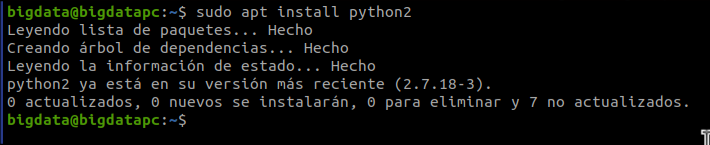
\includegraphics[width=0.8\textwidth]{figures/2.png}
    \caption{Instalación de Python 2}
\end{figure}

Después, descargaremos el archivo .tar.gz de Cassandra desde la página oficial de Apache. Para ello, ejecutamos el siguiente comando:

\begin{lstlisting}[language=bash]
    wget https://dlcdn.apache.org/cassandra/3.11.16/apache-cassandra-3.11.16-bin.tar.gz
\end{lstlisting}

\begin{figure}[H]
    \centering
    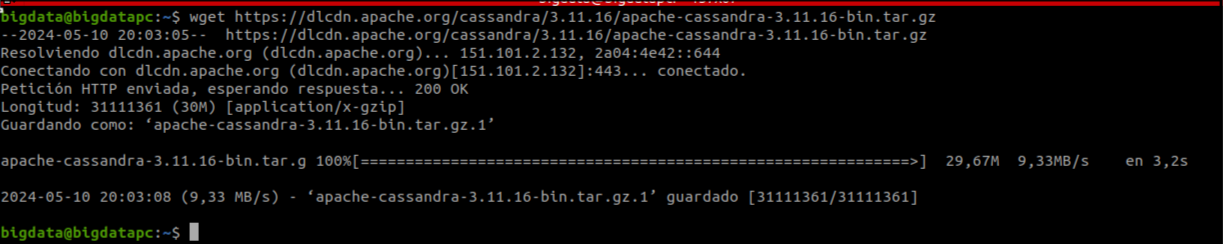
\includegraphics[width=0.8\textwidth]{figures/3.png}
    \caption{Descarga de Cassandra}
\end{figure}

Descomprimimos el archivo .tar.gz con el siguiente comando:

\begin{lstlisting}[language=bash]
    tar -xvzf apache-cassandra-3.11.16-bin.tar.gz
\end{lstlisting}

\begin{figure}[H]
    \centering
    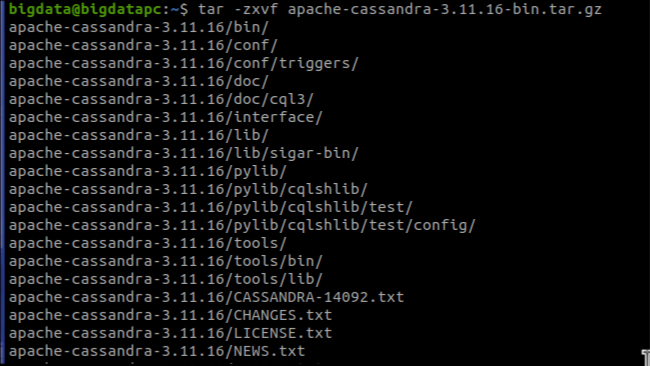
\includegraphics[width=0.8\textwidth]{figures/4.png}
    \caption{Descompresión de Cassandra}
\end{figure}

Por último, eliminamos el archivo .tar.gz con el siguiente comando:

\begin{lstlisting}[language=bash]
    rm apache-cassandra-3.11.16-bin.tar.gz
\end{lstlisting}

\begin{figure}[H]
    \centering
    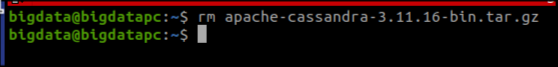
\includegraphics[width=0.8\textwidth]{figures/5.png}
    \caption{Eliminación del archivo .tar.gz}
\end{figure}

\section{Desplegar HDFS}

HDFS ya está instalado por defecto en la máquina virtual en la carpeta \texttt{~/hadoop-3.3.6}. Para desplegar HDFS ejecutamos el siguiente comando:

\begin{lstlisting}[language=bash]
    ~/hadoop-3.3.6/sbin/start-dfs.sh
\end{lstlisting}

\begin{figure}[H]
    \centering
    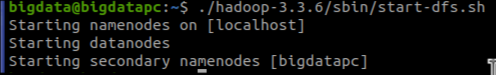
\includegraphics[width=0.8\textwidth]{figures/6.png}
    \caption{Despliegue de HDFS}
\end{figure}

Ahora para comprobar que HDFS se ha desplegado correctamente, ejecutamos el siguiente comando:

\begin{lstlisting}[language=bash]
    jps
\end{lstlisting}

\begin{figure}[H]
    \centering
    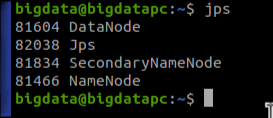
\includegraphics[width=0.8\textwidth]{figures/7.png}
    \caption{Comprobación de HDFS}
\end{figure}

Ahora ya podemos ejecutar comandos de HDFS, como por ejemplo el siguiente comando que muestra los archivos en el sistema de archivos HDFS:

\begin{lstlisting}[language=bash]
    ~/hadoop-3.3.6/bin/hdfs dfs -ls /
\end{lstlisting}

\begin{figure}[H]
    \centering
    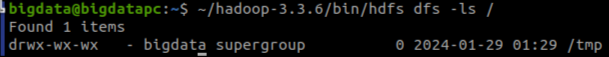
\includegraphics[width=0.8\textwidth]{figures/8.png}
    \caption{Comando de HDFS}
\end{figure}

\section{Desplegar PostgreSQL}

Postgres también está instalado por defecto en la máquina virtual, además se arranca por defecto al iniciar la sesión en la máquina virtual. El motivo por el que arranca por defecto es que se ha configurado como un servicio de systemd, por lo que se inicia automáticamente al arrancar el sistema.

Para comprobar que Postgres se ha desplegado correctamente, ejecutamos el siguiente comando:

\begin{lstlisting}[language=bash]
    sudo systemctl status postgresql
\end{lstlisting}

\begin{figure}[H]
    \centering
    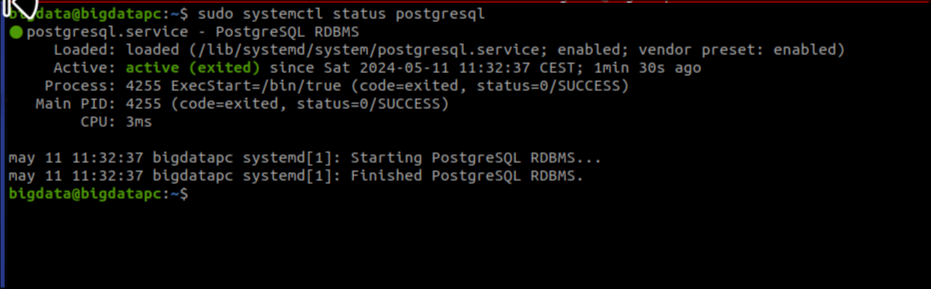
\includegraphics[width=0.8\textwidth]{figures/9.png}
    \caption{Comprobación de Postgres}
\end{figure}

Ahora para asegurarnos de que todo funciona correctamente, nos conectamos a la consola de Postgres y ejecutamos un comando de prueba. Para ello, ejecutamos el siguiente comando:

\begin{lstlisting}[language=bash]
    sudo -u postgres psql
\end{lstlisting}

\begin{lstlisting}[language=sql]
    SELECT version();
\end{lstlisting}

\begin{figure}[H]
    \centering
    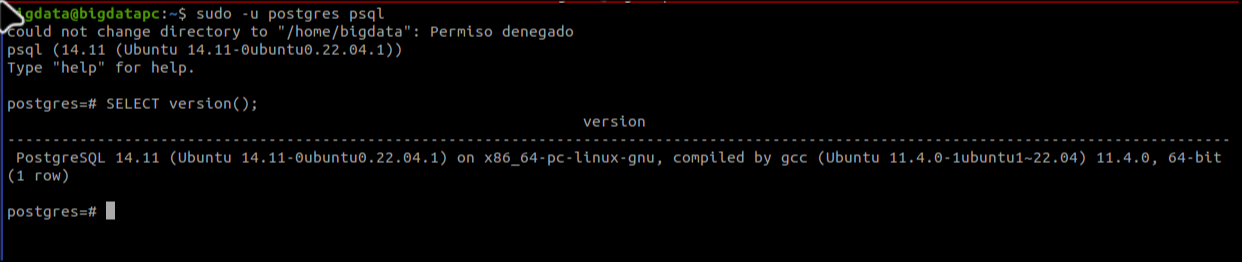
\includegraphics[width=0.8\textwidth]{figures/10.png}
    \caption{Comando de prueba de Postgres}
\end{figure}

\section{Desplegar Cassandra}

Primero nos moveremos a la carpeta de Cassandra con el siguiente comando:

\begin{lstlisting}[language=bash]
    cd ~/apache-cassandra-3.11.16
\end{lstlisting}

Acto seguido, arrancamos el servicio de Cassandra con el siguiente comando:

\begin{lstlisting}[language=bash]
    bin/cassandra
\end{lstlisting}

\begin{figure}[H]
    \centering
    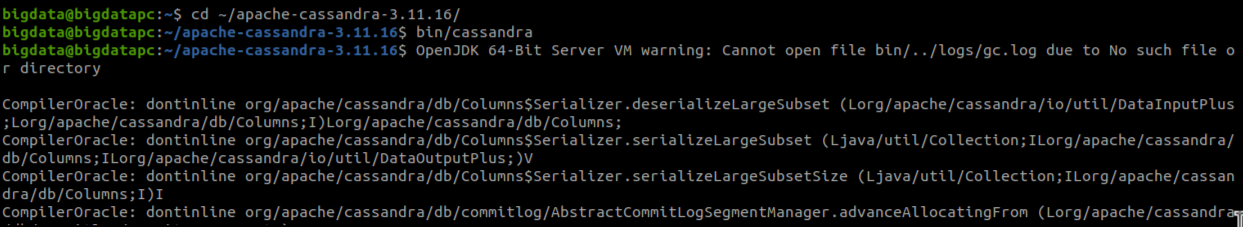
\includegraphics[width=0.8\textwidth]{figures/11.png}
    \caption{Despliegue de Cassandra}
\end{figure}

Ahora inciamos la consola de Cassandra con el siguiente comando:

\begin{lstlisting}[language=bash]
    bin/cqlsh
\end{lstlisting}

\begin{figure}[H]
    \centering
    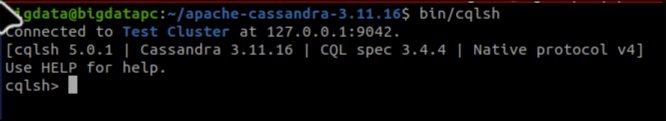
\includegraphics[width=0.8\textwidth]{figures/12.png}
    \caption{Consola de Cassandra}
\end{figure}

Por último, tendremos que generar un keyspace que nos servirá más adelante.

\begin{lstlisting}[language=sql]
    CREATE KEYSPACE IF NOT EXISTS practica WITH REPLICATION = {'class': 'SimpleStrategy', 'replication_factor': 1};
\end{lstlisting}

Salimos de la consola de Cassandra con el siguiente comando:

\begin{lstlisting}[language=sql]
    exit
\end{lstlisting}

\begin{figure}[H]
    \centering
    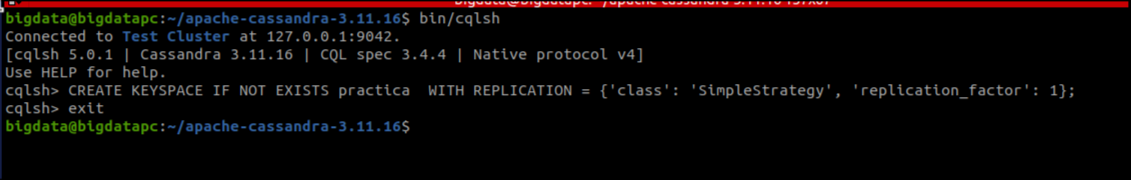
\includegraphics[width=0.8\textwidth]{figures/13.png}
    \caption{Creación de keyspace en Cassandra}
\end{figure}

\section{Desplegar clúster de Spark Standalone}

Vamos a ver como configurar y arrancar un despliegue de 1 nodo Master y 2 nodos Worker de Spark Standalone.

Primero, nos movemos a la carpeta de Spark con el siguiente comando:

\begin{lstlisting}[language=bash]
    cd ~/spark-3.3.3-bin-hadoop3
\end{lstlisting}

\begin{figure}[H]
    \centering
    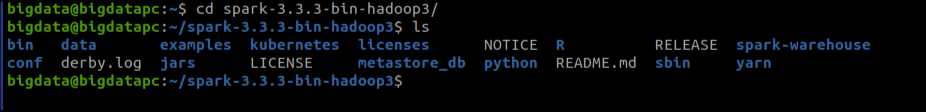
\includegraphics[width=0.8\textwidth]{figures/14.png}
    \caption{Cambio de directorio a Spark}
\end{figure}

Una vez que estamos en la carpeta de Spark, arrancamos el Master con el siguiente comando:

\begin{lstlisting}[language=bash]
    sbin/start-master.sh
\end{lstlisting}

\begin{figure}[H]
    \centering
    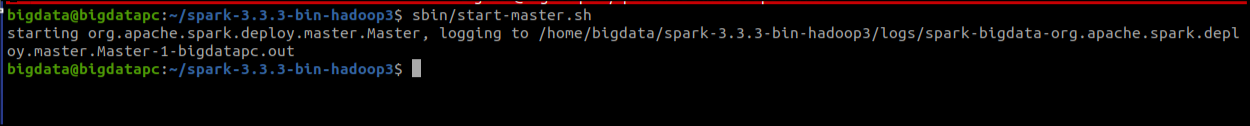
\includegraphics[width=0.8\textwidth]{figures/15.png}
    \caption{Arranque del Master de Spark}
\end{figure}

En la ejecución del comando anterior, se nos muestra el archivo de los logs del Master, en este caso el archivo es \textit{/home/bigdata/spark-3.3.3-bin-hadoop3/logs/spark-bigdata-org.apache.spark.deploy.master.Master-1-bigdatac.out}. Con un par de comandos sacaremos la URL del Master, que es la dirección que usaremos para conectarnos a la interfaz web del Master.

\begin{lstlisting}[language=bash]
    cat /home/bigdata/spark-3.3.3-bin-hadoop3/logs/spark-bigdata-org.apache.spark.deploy.master.Master-1-bigdatac.out | grep 'http://' | awk '{print $NF}'
\end{lstlisting}

\begin{figure}[H]
    \centering
    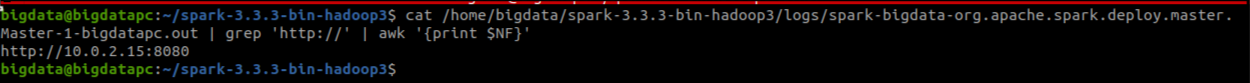
\includegraphics[width=0.8\textwidth]{figures/16.png}
    \caption{URL del Master de Spark}
\end{figure}

En nuestro caso, si nos conectamos a la URL \texttt{http://10.0.2.15:8080/} podremos ver la interfaz web del Master de Spark.

\begin{figure}[H]
    \centering
    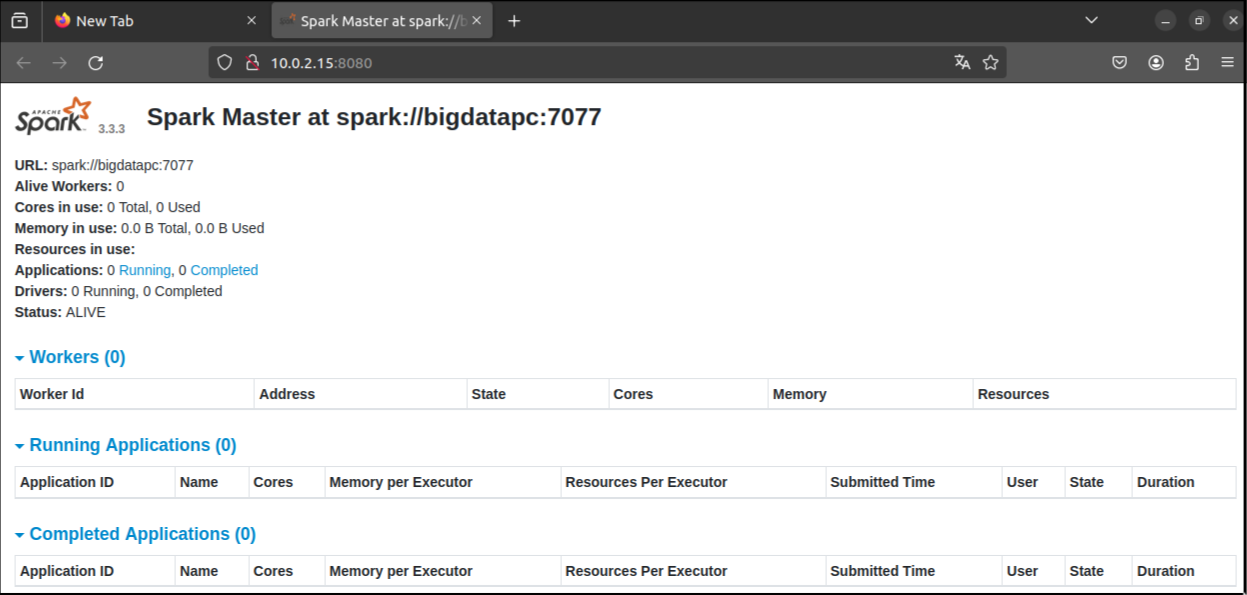
\includegraphics[width=0.8\textwidth]{figures/17.png}
    \caption{Interfaz web del Master de Spark}
\end{figure}

Para los workes, también necesitaremos una URL que encontraremos en los logs del Master. Para ello, ejecutamos el siguiente comando:

\begin{lstlisting}[language=bash]
    cat /home/bigdata/spark-3.3.3-bin-hadoop3/logs/spark-bigdata-org.apache.spark.deploy.master.Master-1-bigdatac.out | grep 'spark://' | awk '{print $NF}'
\end{lstlisting}

\begin{figure}[H]
    \centering
    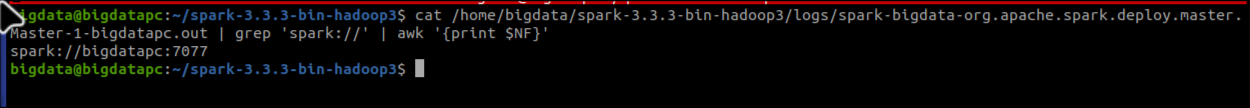
\includegraphics[width=0.8\textwidth]{figures/18.png}
    \caption{URL de los Workers de Spark}
\end{figure}

Antes de desplegar los Workres, para poder tener dos Workers en una misma máquina vamos a modificar la configuración del archivo \texttt{conf/spark-env.sh}. Para ello, ejecutamos el siguiente comando:

\begin{lstlisting}[language=bash]
    vim conf/spark-env.sh
\end{lstlisting}

Y añadimos las 3 siguientes líneas al final del archivo:

\begin{lstlisting}[language=bash]
    SPARK_WORKER_INSTANCES=2
    SPARK_WORKER_CORES=2
    SPARK_WORKER_MEMORY=1g
\end{lstlisting}

\begin{figure}[H]
    \centering
    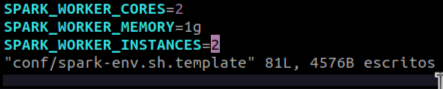
\includegraphics[width=0.8\textwidth]{figures/20.png}
    \caption{Configuración de los Workers de Spark}
\end{figure}

Ahora arrancaremos dos Workers con 1GB de memoria y 2 cores (la configuración que hemos especificado). Es necesario especificar la memoria y los cores ya que por defecto los Workers usarán toda la memoria y todos los cores disponibles.

\begin{lstlisting}[language=bash]
    sbin/start-slave.sh spark://bigdatapc:7077
\end{lstlisting}

\begin{figure}[H]
    \centering
    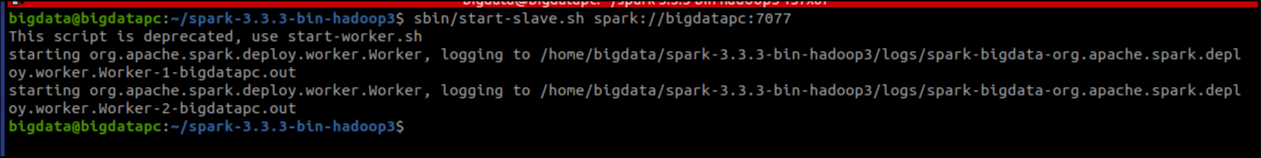
\includegraphics[width=0.8\textwidth]{figures/19.png}
    \caption{Arranque de los Workers de Spark}
\end{figure}

Si nos vamos a la interfaz web del Master de Spark, podremos ver los Workers conectados. En esta interfaz se nos muestra el id del nodo Worker, la dirección IP, el número de cores, la memoria disponible, la carga de trabajo, la memoria utilizada y el estado del nodo. Además, arriba se nos muestra un resumen de todos los recursos usados y de las aplicaciones en ejecución.

\begin{figure}[H]
    \centering
    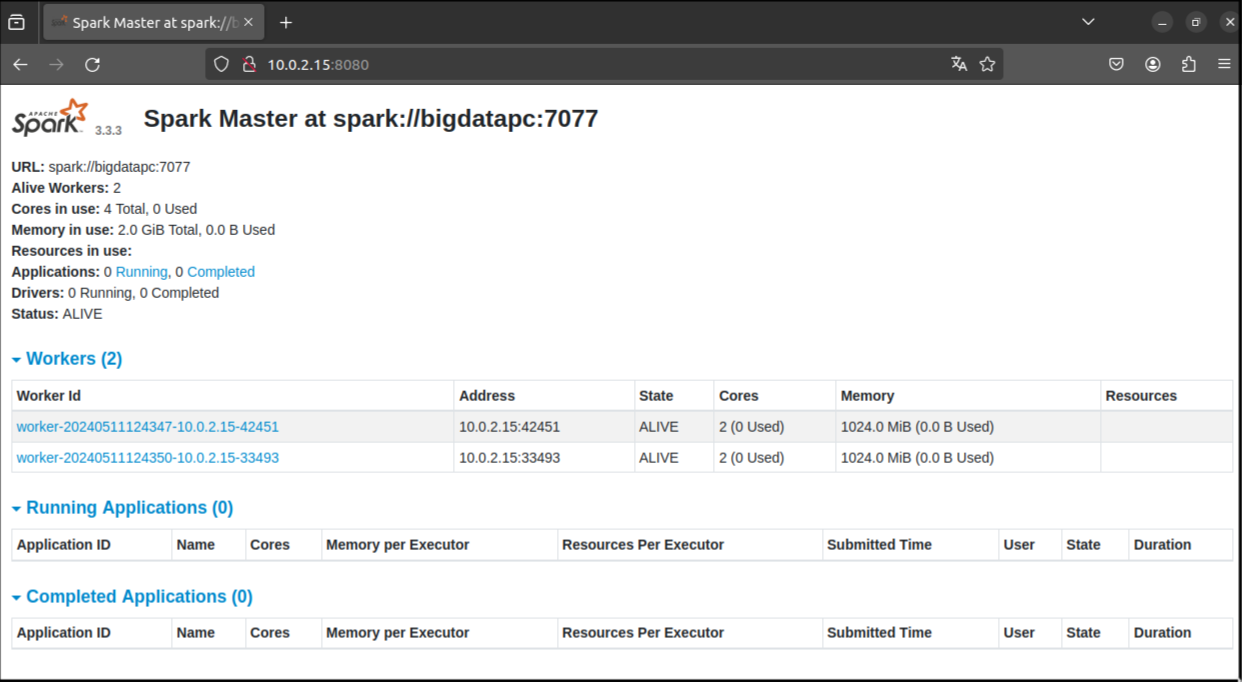
\includegraphics[width=0.8\textwidth]{figures/21.png}
    \caption{Interfaz web del Master de Spark con los Workers conectados}
\end{figure}

\section{Desplegar una shell de Spark}

El primer paso será descargar los conectores de Postgres y Cassandra. Primero nos moveremos a la carpeta \textit{spark-3.3.3-bin-hadoop3/jars} y a continuación descargaremos los conectores con los siguientes comandos:

\begin{lstlisting}[language=bash]
    cd ~/spark-3.3.3-bin-hadoop3/jars
    wget https://jdbc.postgresql.org/download/postgresql-42.7.3.jar
    wget https://repo1.maven.org/maven2/com/datastax/spark/spark-cassandra-connector_2.12/3.3.0/spark-cassandra-connector_2.12-3.3.0.jar
\end{lstlisting}

\begin{figure}[H]
    \centering
    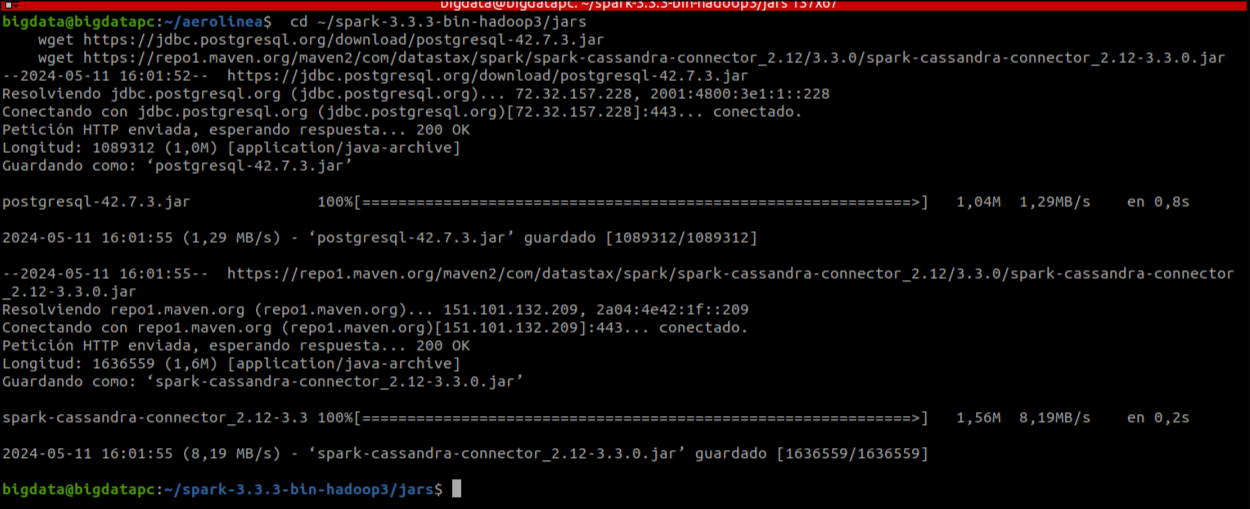
\includegraphics[width=0.8\textwidth]{figures/22.png}
    \caption{Descarga de los conectores de Postgres y Cassandra}
\end{figure}

Ahora, para arrancar una shell de Spark, ejecutaremos el siguiente comando. En este comando especificamos la memoria que queremos que use el driver y los executors, así como el número de cores que queremos que use el driver y los executors. Además, especificamos los conectores que hemos descargado anteriormente.

\begin{lstlisting}[language=bash]
bin/spark-shell --master spark://bigdatapc:7077 --driver-memory 1G --executor-memory 1G --total-executor-cores 2 --executor-cores 2 --jars jars/postgresql-42.7.3.jar,jars/spark-cassandra-connector_2.12-3.3.0.jar
\end{lstlisting}

\begin{figure}[H]
    \centering
    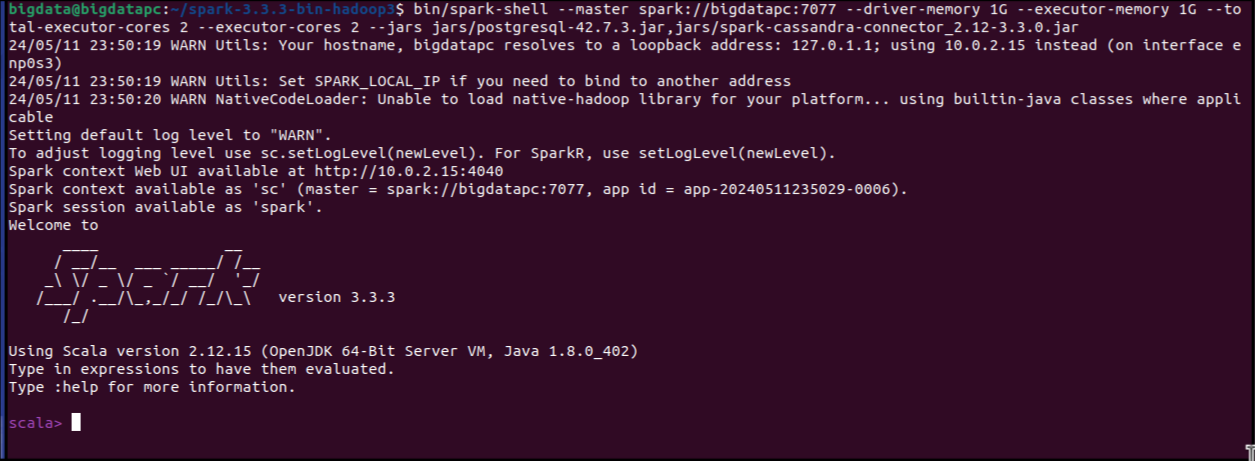
\includegraphics[width=0.8\textwidth]{figures/23.png}
    \caption{Arranque de la shell de Spark}
\end{figure}

Si vamos a la web, veremos que se ha creado una aplicación en la interfaz web del Master de Spark.

\begin{figure}[H]
    \centering
    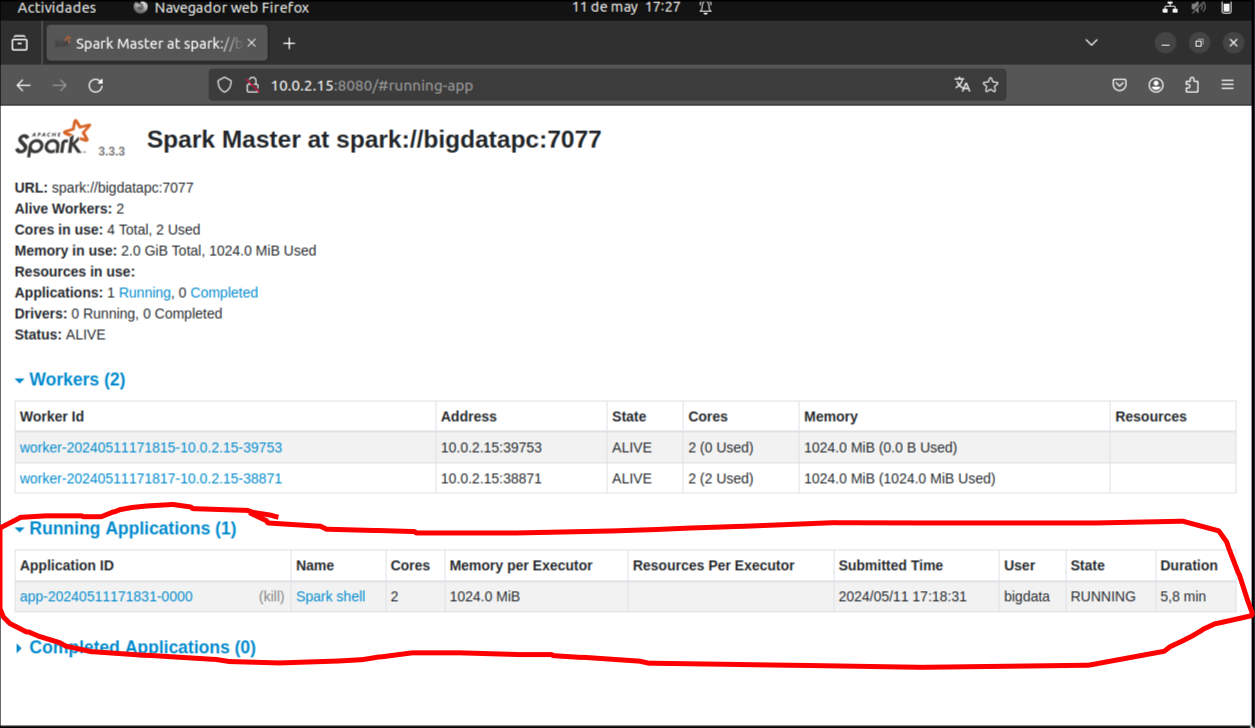
\includegraphics[width=0.8\textwidth]{figures/24.png}
    \caption{Interfaz web del Master de Spark con la aplicación creada}
\end{figure}

También, al arrancar la shell de Spark, se nos muestra la URL de la interfaz web de la shell de Spark:

\begin{figure}[H]
    \centering
    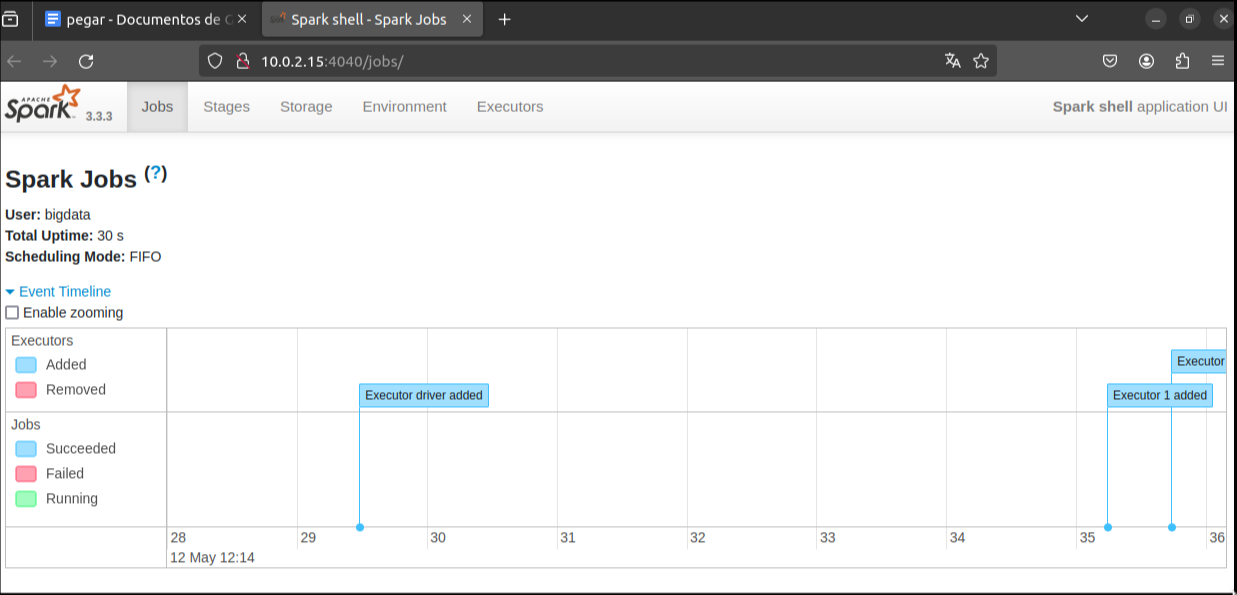
\includegraphics[width=0.8\textwidth]{figures/58.png}
    \caption{Interfaz web de la shell de Spark}
\end{figure}

\chapter{Ingesta de los datos en el lago de datos}

Los datos que se van a analizar en este trabajo han sido proporcionados por el profesor en el archivo \texttt{datos_practica.tar.gz}. El primer paso es descomprimir el archivo y ver qué contiene. Para ello, se ejecuta el siguiente comando en la terminal:

\begin{lstlisting}[language=bash]
tar -xvzf datos_practica.tar.gz
\end{lstlisting}

Ahora desde la consola de Spark iremos cargando los datos en el lago de datos.

\section{Countries}

Los datos sobre los paises en el archivo \texttt{countries.txt} está en un formato no estándar: \texttt{name::<name> \#\# iso_code::<iso_code> \#\# dafif_code::<dafif_code>}, por lo que se va a tener que tratar como datos desectructurados (RDDs) y realizar una serie de trnsformaciones con el objetivo de realizar una limpieza de los datos y darle una estructura \texttt{name: string, iso_code: string,
dafif_code: string} para obtener un DataFrame. Una vez obtenido el Dataframe, se debe utilizar el conector csv para guardar los datos en el path \texttt{/practica/countries/} de HDFS.

Primero introducimos nuestro archivo en un RDD y lo mostramos:

\begin{lstlisting}[language=scala]
val rdd = sc.textFile("/home/bigdata/practica/countries.txt")
rdd.take(5).foreach(println)
\end{lstlisting}

\begin{figure}[H]
    \centering
    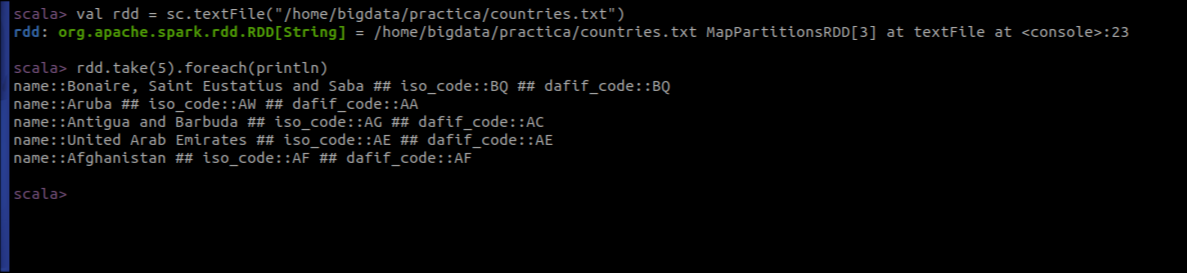
\includegraphics[width=0.8\textwidth]{figures/25.png}
    \caption{RDD de los países}
    \label{fig:countries_rdd}
\end{figure}

Ahora vamos a realizar una serie de transformaciones para limpiar los datos y darles una estructura. Para ello, vamos a utilizar el método \texttt{map} para dividir las líneas por el separador \texttt{\#\#}, eliminar los espacios en blanco y eliminar los elementos vacíos. A continuación, filtramos las líneas que no tengan 3 elementos y mostramos el resultado:

\begin{lstlisting}[language=scala]
val lines = rdd.map(line => line.split("##").map(_.trim).filter(_.nonEmpty)).filter(_.size == 3)
lines.collect()(0)
\end{lstlisting}

\begin{figure}[H]
    \centering
    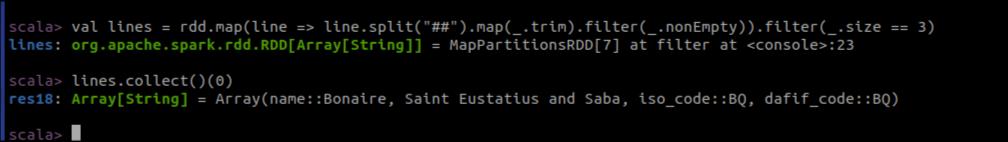
\includegraphics[width=0.8\textwidth]{figures/26.png}
    \caption{RDD de los países limpio}
    \label{fig:countries_rdd_clean}
\end{figure}

Crearemos la variable columnas en la que quitaremos el prefijo de las columnas (ej: \texttt{name::}) y mostraremos el resultado:

\begin{lstlisting}[language=scala]
val columns = lines.map(line => line.map(_.split("::")(1)))
columns.collect()(0)
\end{lstlisting}

\begin{figure}[H]
    \centering
    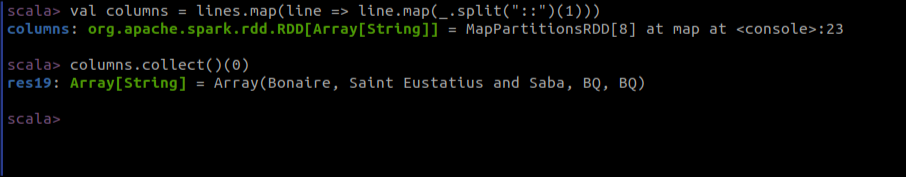
\includegraphics[width=0.8\textwidth]{figures/27.png}
    \caption{RDD de los países con nombres de columnas}
    \label{fig:countries_rdd_columns}
\end{figure}

Ahora ya si crearemos el dataframe de countries:

\begin{lstlisting}[language=scala]
val df_countries = columns.map(row => (row(0), row(1), row(2))).toDF("name", "iso_code", "dafif_code")
df_countries.show()
\end{lstlisting}

\begin{figure}[H]
    \centering
    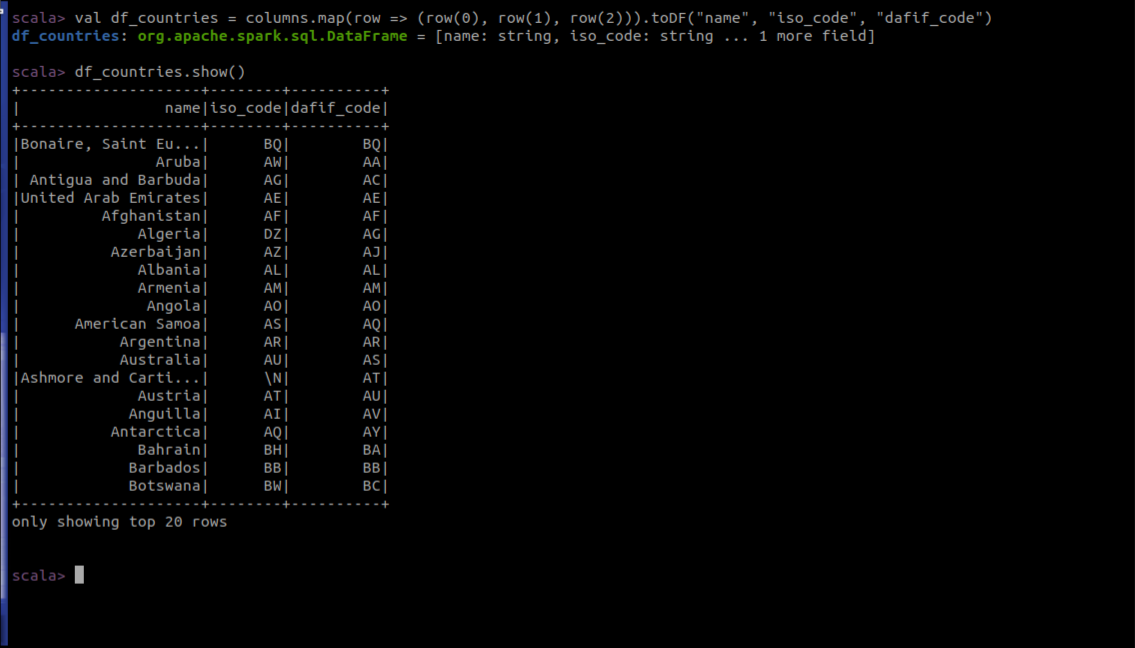
\includegraphics[width=0.8\textwidth]{figures/28.png}
    \caption{Dataframe de los países}
    \label{fig:countries_df}
\end{figure}

Ahora en otra terminal inciamos HDFS.

\begin{lstlisting}[language=bash]
hadoop-3.3.6/sbin/start-dfs.sh
\end{lstlisting}

\begin{figure}[H]
    \centering
    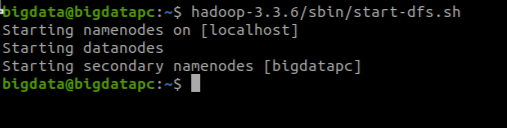
\includegraphics[width=0.8\textwidth]{figures/29.png}
    \caption{Iniciando HDFS}
    \label{fig:start_hdfs}
\end{figure}

Y guardamos el dataframe en HDFS desde la consola de scala:

\begin{lstlisting}[language=scala]
df_countries.write.format("csv").option("header","true").save("hdfs://localhost:9000/practica/countries/")
\end{lstlisting}

\begin{figure}[H]
    \centering
    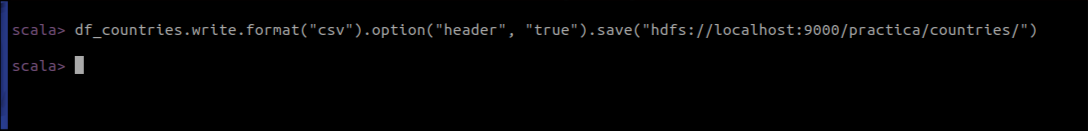
\includegraphics[width=0.8\textwidth]{figures/30.png}
    \caption{Guardando el dataframe en HDFS}
    \label{fig:save_df}
\end{figure}

Mostramos el contenido de la carpeta \texttt{/practica/countries/} en HDFS:

\begin{lstlisting}[language=bash]
hadoop-3.3.6/bin/hdfs dfs -ls /practica/countries/
\end{lstlisting}

\begin{figure}[H]
    \centering
    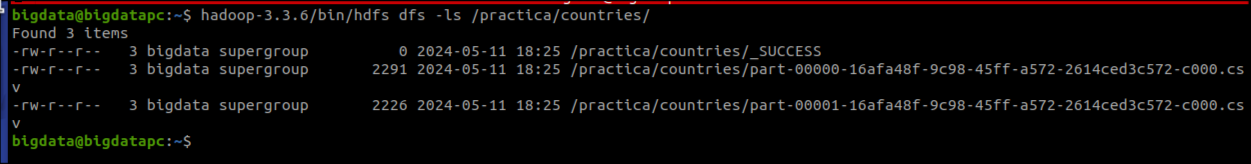
\includegraphics[width=0.8\textwidth]{figures/31.png}
    \caption{Contenido de la carpeta countries en HDFS}
    \label{fig:countries_hdfs}
\end{figure}

Por último, mostraremos 5 filas de los datos almacenados en HDFS:

\begin{lstlisting}[language=scala]
spark.read.format("csv").option("header", "true").option("inferSchema","true").load("hdfs://localhost:9000/practica/countries/").limit(5).show()
\end{lstlisting}

\begin{figure}[H]
    \centering
    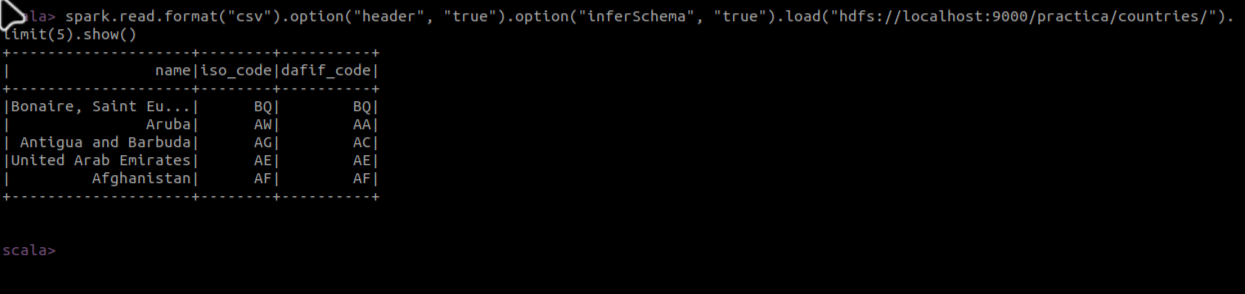
\includegraphics[width=0.8\textwidth]{figures/32.png}
    \caption{5 filas de los datos almacenados en HDFS}
    \label{fig:countries_hdfs_data}
\end{figure}

\section{Airlines}

Los datos sobre las aerolíneas están en el archivo \texttt{airlines.dat} y está en formato CSV. Por lo tanto, al ser datos estructurados, se puede cargar directamente en un DataFrame. Una de las columnas require una transformación ya que debería ser booleana en vez de string. Además, se nos pide añadir una columna nueva llamada \texttt{country_iso} que corresponde al \textit{iso_code} de los datos CSV que guardamos en HDFS. Una vez terminado, se debe utilizar el conector \textit{parquet} para guardar los datos particionados por la columna \textit{country} en el path \texttt{/practica/airlines/} de HDFS.

Primero cargamos los datos de airlines.dat en un Dataframe a través del conector de csv y las propiedades necesarias, para ello comenzaremos importando algunas estructuras de datos:

\begin{lstlisting}[language=scala]
import org.apache.spark.sql.types.StructType
import org.apache.spark.sql.types.StructField
import org.apache.spark.sql.types.StringType
import org.apache.spark.sql.types.IntegerType
import org.apache.spark.sql.types.FloatType
\end{lstlisting}

\begin{figure}[H]
    \centering
    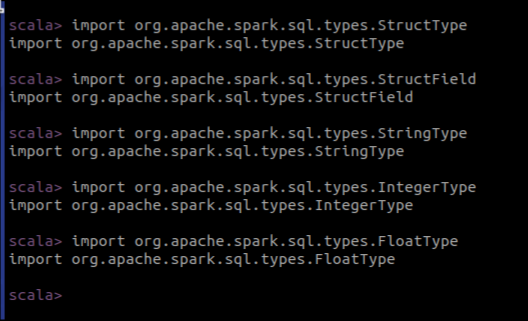
\includegraphics[width=0.8\textwidth]{figures/33.png}
    \caption{Importando estructuras de datos}
    \label{fig:import_data_structures}
\end{figure}

Después creamos un esquema para los datos de las aerolíneas:

\begin{lstlisting}[language=scala]
val airlines_schema = StructType(Array(StructField("id", IntegerType, true), StructField("name", StringType, true), StructField("alias", StringType,true), StructField("IATA", StringType, true),StructField("ICAO", StringType, true),StructField("callsign", StringType, true), StructField("country", StringType, true), StructField("active", StringType, true)))
\end{lstlisting}

\begin{figure}[H]
    \centering
    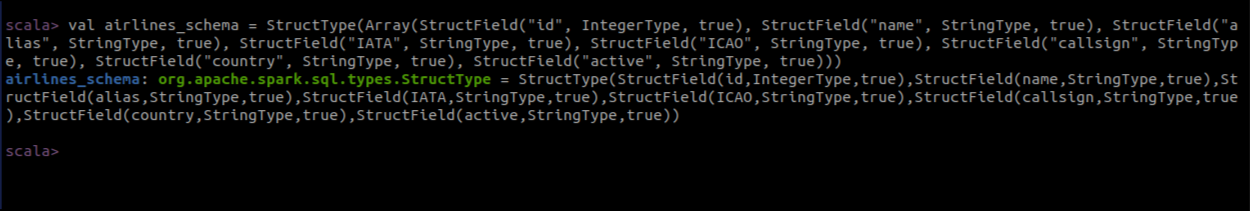
\includegraphics[width=0.8\textwidth]{figures/34.png}
    \caption{Creando el esquema de los datos de las aerolíneas}
    \label{fig:create_airlines_schema}
\end{figure}

Cargamos los datos en un DataFrame utilizando el esquema creado:

\begin{lstlisting}[language=scala]
var df_airlines = spark.read.format("csv").option("header", "false").schema(airlines_schema).load("/home/bigdata/practica/airlines.dat")
df_airlines.show()
\end{lstlisting}

\begin{figure}[H]
    \centering
    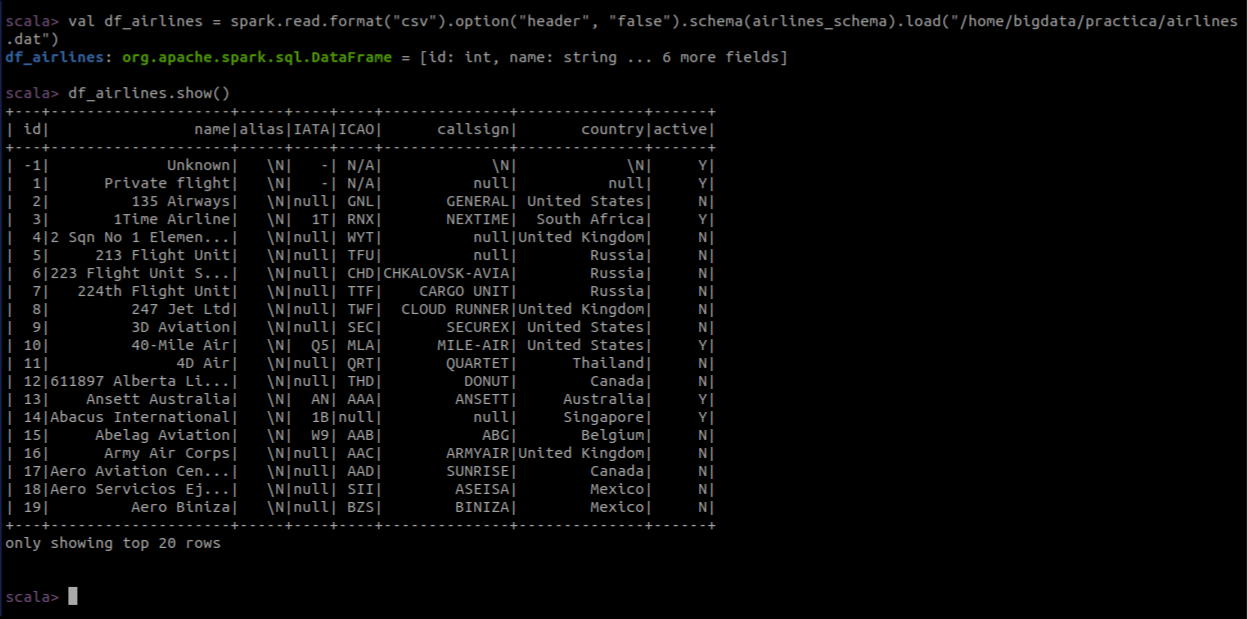
\includegraphics[width=0.8\textwidth]{figures/35.png}
    \caption{Dataframe de las aerolíneas}
    \label{fig:airlines_df}
\end{figure}

Ahora realizaremos las transformaciones necesarias para convertir los datos y el tipo de la columna active de String a Boolean

\begin{lstlisting}[language=scala]
    df_airlines = df_airlines.withColumn("active", when(col("active") === "Y", true).otherwise(false))
\end{lstlisting}

\begin{figure}[H]
    \centering
    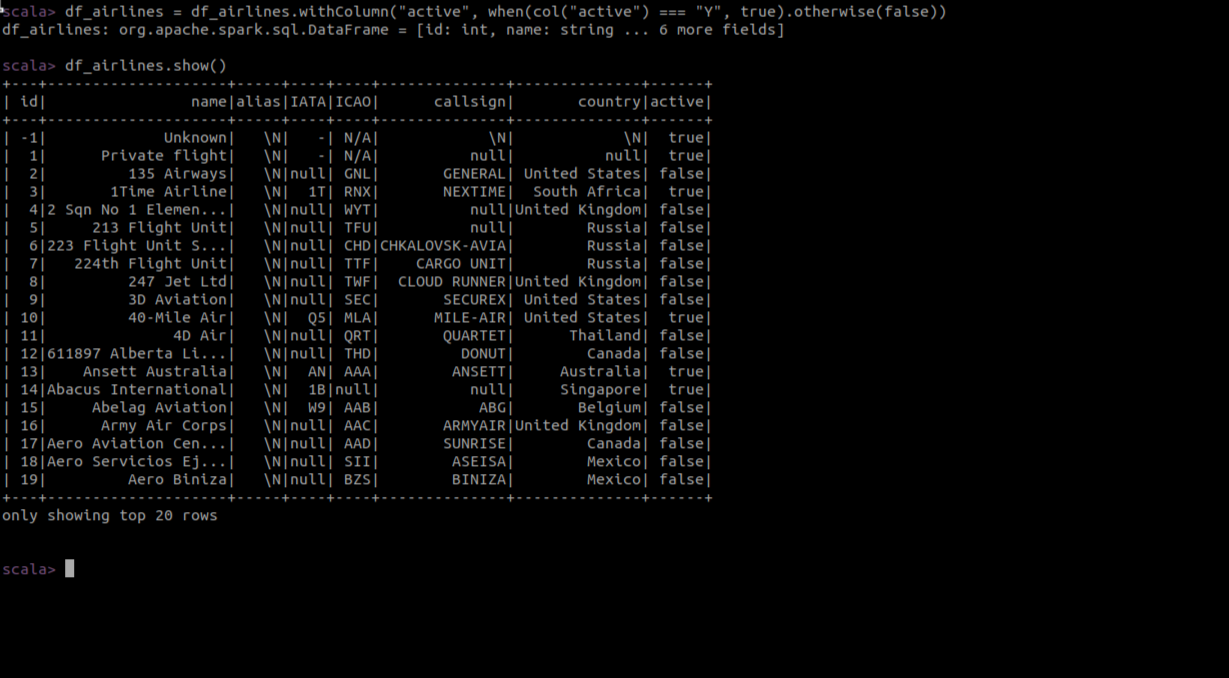
\includegraphics[width=0.8\textwidth]{figures/36.png}
    \caption{Dataframe de las aerolíneas con la columna active convertida a boolean}
    \label{fig:airlines_df_active}
\end{figure}

Ahora cargaremos los datos de los países en un DataFrame para poder unirlo con el DataFrame de las aerolíneas:

\begin{lstlisting}[language=scala]
var df_countries = spark.read.format("csv").option("header","true").option("inferSchema", "true").load("hdfs://localhost:9000/practica/countries/")
countries.show()
\end{lstlisting}

\begin{figure}[H]
    \centering
    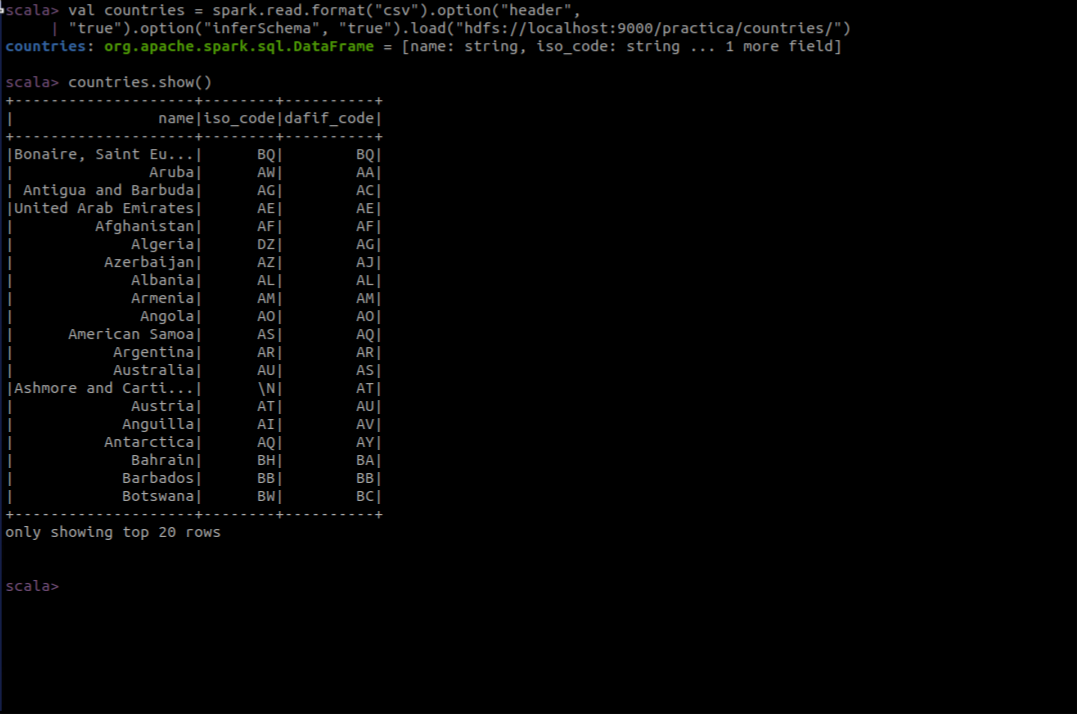
\includegraphics[width=0.8\textwidth]{figures/37.png}
    \caption{Dataframe de los países}
    \label{fig:countries_df_from_hdfs}
\end{figure}

Como \texttt{countries} y \texttt{df\_airlines} tienen una columna en común, \texttt{country}, tenemos que renombrar la columna \texttt{name} de countries a \texttt{country} para poder unir los dos DataFrames.

\begin{lstlisting}[language=scala]
df_countries = df_countries.withColumnRenamed("name", "country")
\end{lstlisting}

Ahora unimos los dos DataFrames por la columna \texttt{country} y renombramos la columna \texttt{iso_code} a \texttt{country_iso}:

\begin{lstlisting}[language=scala]
df_airlines = df_airlines.join(df_countries, Seq("country"), "left")
df_airlines = df_airlines.withColumnRenamed("iso_code", "country_iso")
\end{lstlisting}

\begin{figure}[H]
    \centering
    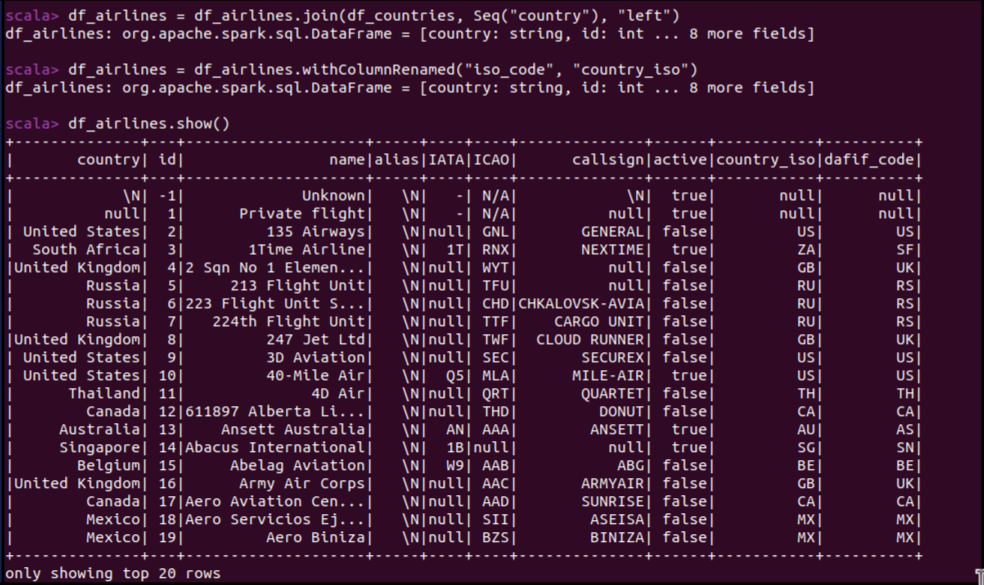
\includegraphics[width=0.8\textwidth]{figures/38.png}
    \caption{Dataframe de las aerolíneas con los países}
    \label{fig:airlines_countries_df}
\end{figure}

Vamos a eliminar la columna \texttt{darif_code} ya que no la necesitamos:

\begin{lstlisting}[language=scala]
df_airlines = df_airlines.drop("dafif_code")
\end{lstlisting}

También reordenaremos las columnas para que \texttt{id} sea la primera columna:

\begin{lstlisting}[language=scala]
df_airlines = df_airlines.select("id", "name", "alias", "IATA", "ICAO", "callsign", "country", "country_iso", "active")
\end{lstlisting}

\begin{figure}[H]
    \centering
    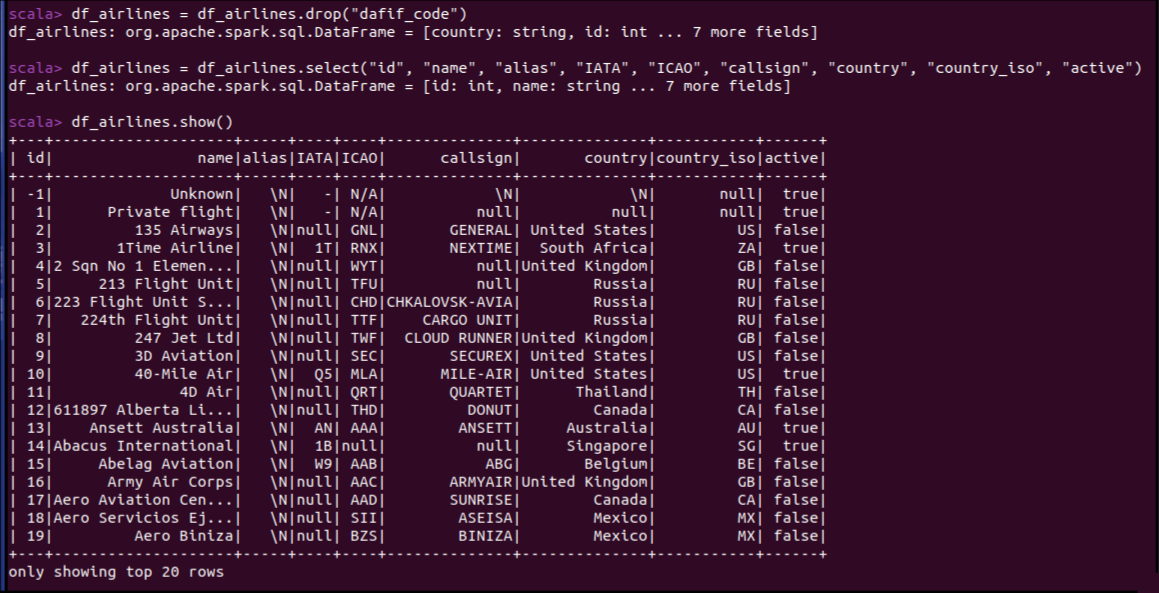
\includegraphics[width=0.8\textwidth]{figures/39.png}
    \caption{Dataframe de las aerolíneas con las columnas reordenadas}
    \label{fig:airlines_reordered_df}
\end{figure}

Vamos a eliminar las filas que tengan valores nulos o \texttt{\textbackslash N} en la columna \texttt{country}:

\begin{lstlisting}[language=scala]
df_airlines = df_airlines.filter(col("country").isNotNull && col("country") =!= "\\N"))
\end{lstlisting}

\begin{figure}[H]
    \centering
    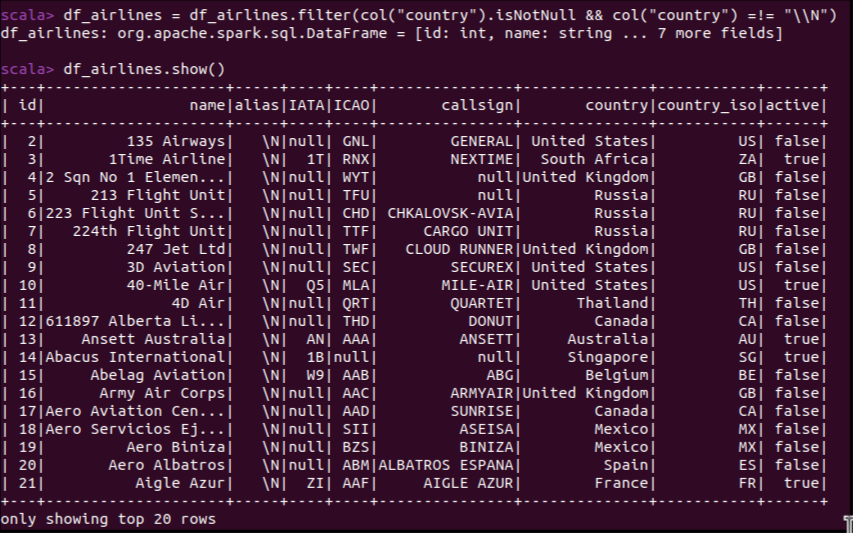
\includegraphics[width=0.8\textwidth]{figures/40.png}
    \caption{Dataframe de las aerolíneas sin valores nulos en la columna country}
    \label{fig:airlines_no_null_df}
\end{figure}

Por último, guardamos el DataFrame en HDFS particionado por la columna \texttt{country}:

\begin{lstlisting}[language=scala]
df_airlines.write.format("parquet").partitionBy("country").save("hdfs://localhost:9000/practica/airlines/")
\end{lstlisting}

Cargramos los datos de las aerolíneas desde HDFS y mostramos 5 filas:

\begin{lstlisting}[language=scala]
spark.read.format("parquet").load("hdfs://localhost:9000/practica/airlines/").limit(5).show()
\end{lstlisting}

\begin{figure}[H]
    \centering
    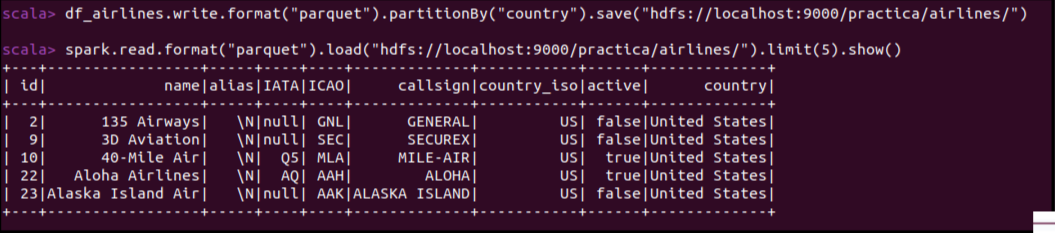
\includegraphics[width=0.8\textwidth]{figures/41.png}
    \caption{5 filas de los datos de las aerolíneas en HDFS}
    \label{fig:airlines_hdfs_data}
\end{figure}

\section{Airports}

Los datos sobre aeropuertos (fichero \texttt{airports.dat}) están en formato CSV. Por tanto, estos datos se pueden cargar en un Dataframe con el conector correspondiente y las opciones que se requieran. Una de las columnas está en una unidad de medida que no es compatible con los sistemas del cliente. Esa columna es \texttt{altitude} y sus valores están en pies. Para realizar la transformación a metros, se debe desarrollar una UDF y ser aplicada en dicha columna. Una vez obtenido este Dataframe, se debe utilizar el conector JDBC para guardar los datos en la tabla airports de Postgres. Además, el líder técnico de nuestro proyecto indica que, al hacer la lectura de estos datos, se deben añadir las propiedades \texttt{partitionColumn}, \texttt{lowerBound}, \texttt{upperBound} y \texttt{numPartitions} propias del conector JDBC.

Creamos el esquema de los datos de los aeropuertos:

\begin{lstlisting}[language=scala]
val airports_schema = StructType(Array(StructField("id", IntegerType, true), StructField("name", StringType, true), StructField("city", StringType, true), StructField("country", StringType, true), StructField("IATA", StringType, true), StructField("ICAO", StringType, true), StructField("latitude", FloatType, true), StructField("longitude", FloatType, true), StructField("altitude", IntegerType, true), StructField("timeZone", FloatType, true), StructField("DST", StringType, true), StructField("tz_database", StringType, true), StructField("tipo", StringType, true), StructField("source", StringType, true)))
\end{lstlisting}

\begin{figure}[H]
    \centering
    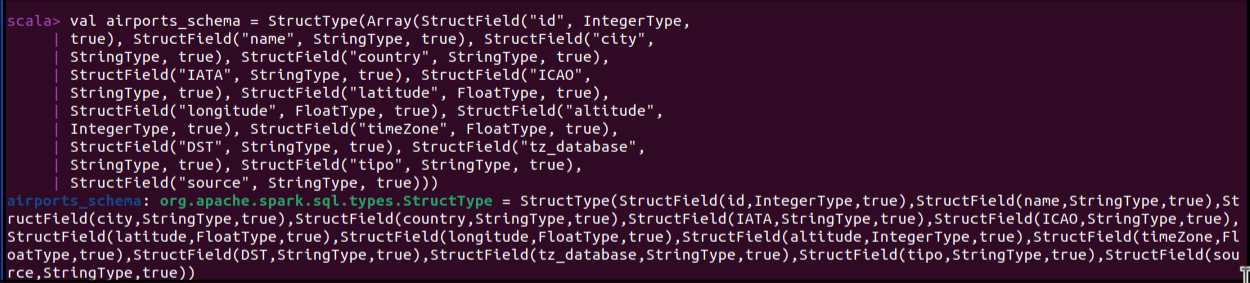
\includegraphics[width=0.8\textwidth]{figures/42.png}
    \caption{Creando el esquema de los datos de los aeropuertos}
    \label{fig:create_airports_schema}
\end{figure}

Cargamos los datos en un DataFrame utilizando el esquema creado:

\begin{lstlisting}[language=scala]
var df_airports = spark.read.format("csv").option("header", "false").schema(airports_schema).load("/home/bigdata/practica/airports.dat")
\end{lstlisting}

\begin{figure}[H]
    \centering
    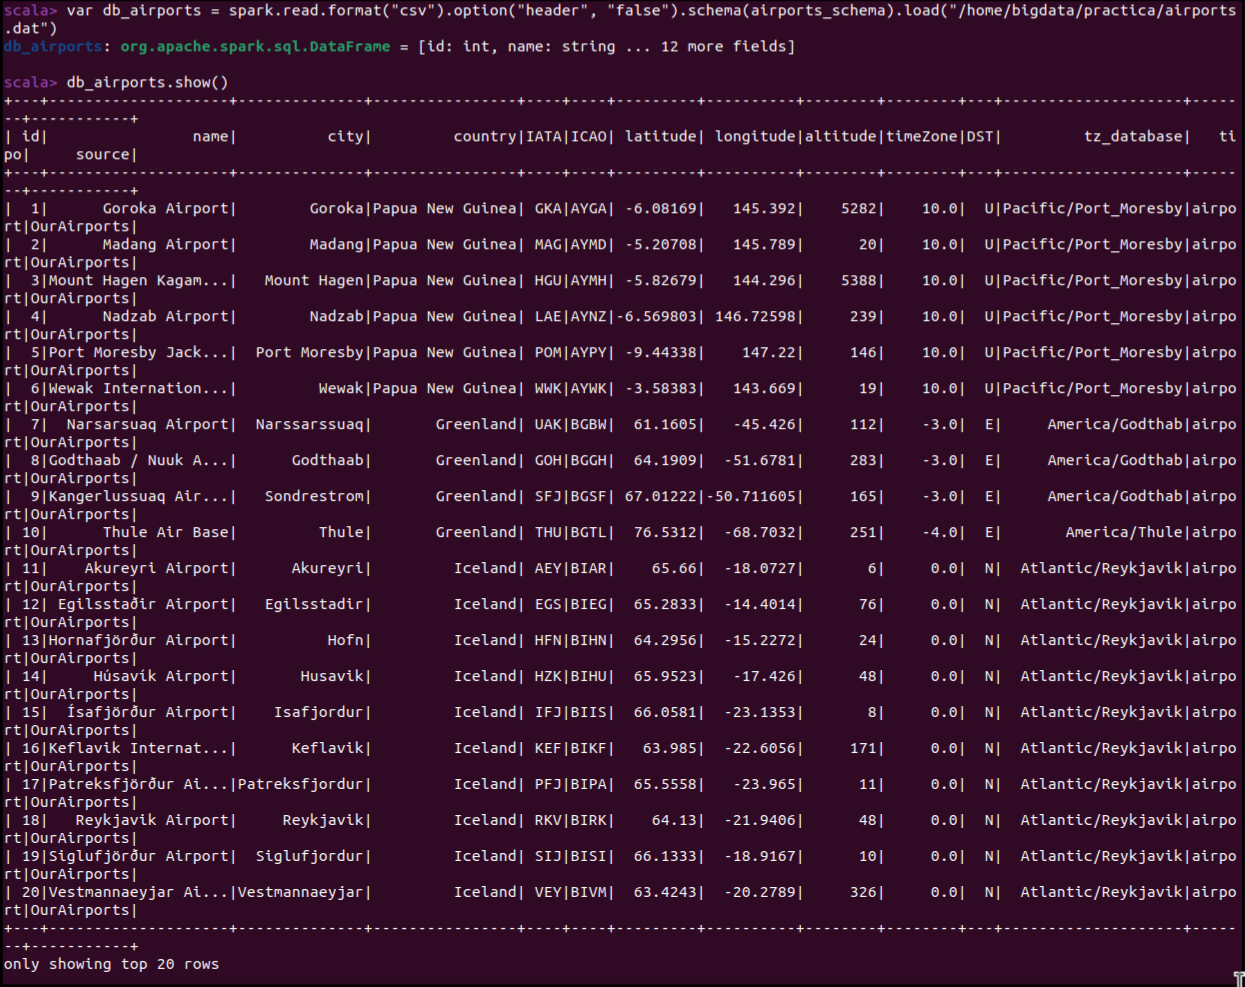
\includegraphics[width=0.8\textwidth]{figures/43.png}
    \caption{Dataframe de los aeropuertos}
    \label{fig:airports_df}
\end{figure}

Ahora haremos la conversión de la columna \texttt{altitude} de pies a metros, primero creamos la variable \texttt{feetToMeters} que será nuestra UDF:

\begin{lstlisting}[language=scala]
val feetToMeters = udf((x: Float) => x / 3.281)
\end{lstlisting}

\begin{figure}[H]
    \centering
    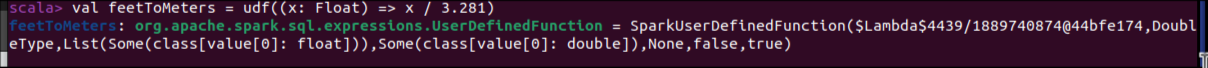
\includegraphics[width=0.8\textwidth]{figures/44.png}
    \caption{Creando la UDF feetToMeters}
    \label{fig:create_udf}
\end{figure}

Y aplicamos la UDF a la columna \texttt{altitude}:

\begin{lstlisting}[language=scala]
df_airports = df_airports.withColumn("altitude", feetToMeters(col("altitude")))
\end{lstlisting}

\begin{figure}[H]
    \centering
    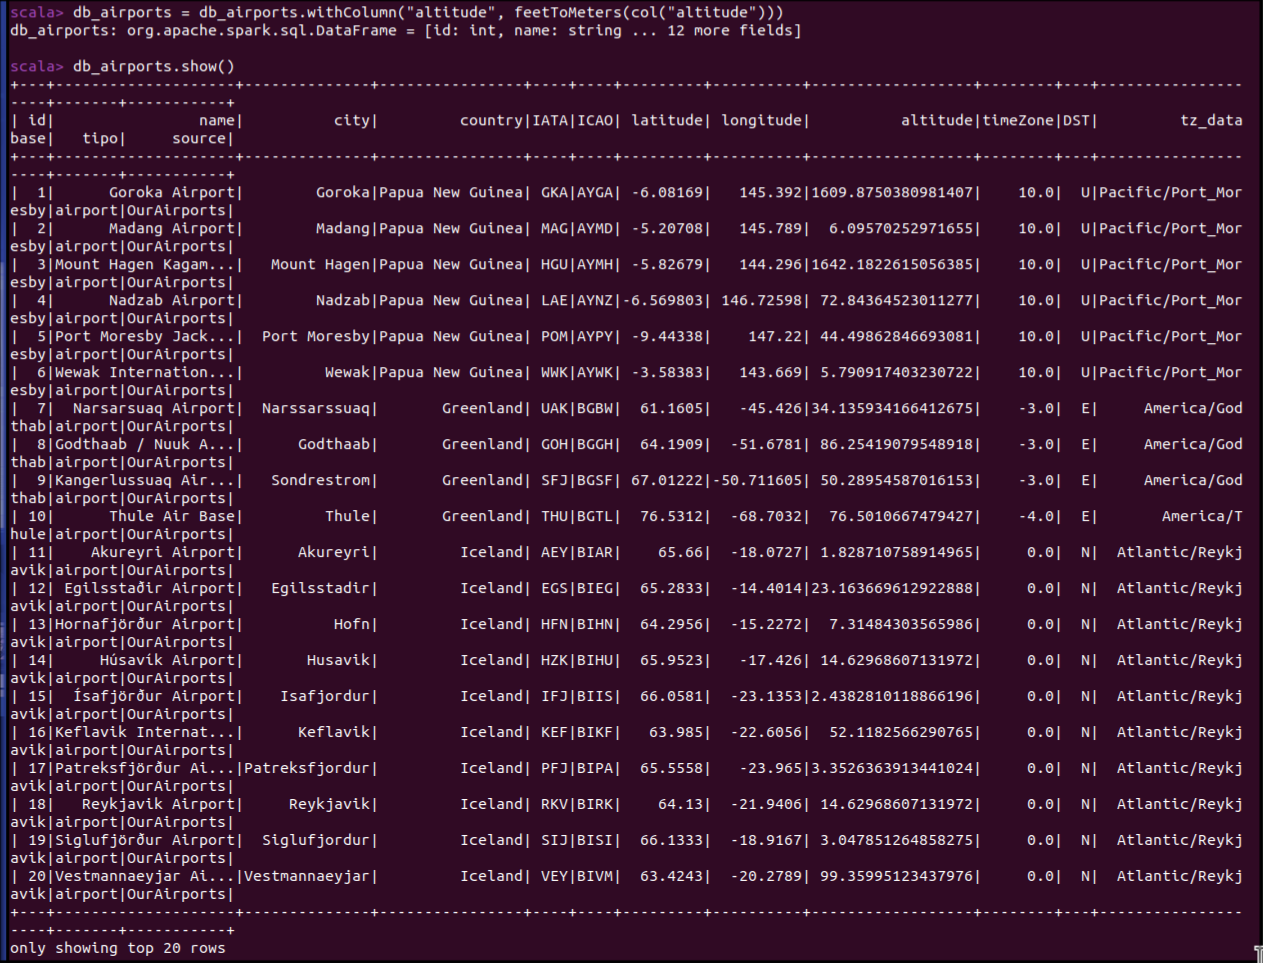
\includegraphics[width=0.8\textwidth]{figures/45.png}
    \caption{Dataframe de los aeropuertos con la columna altitude convertida a metros}
    \label{fig:airports_df_altitude}
\end{figure}

Para poder guardar los datos en la tabla \texttt{airports} de Postgres, primero la tendremos que crear. Primero nos metemos en la consola de Postgres:

\begin{lstlisting}[language=bash]
sudo -u postgres psql
\end{lstlisting}

\begin{figure}[H]
    \centering
    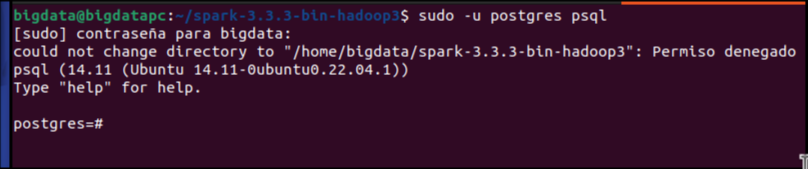
\includegraphics[width=0.8\textwidth]{figures/46.png}
    \caption{Entrando en la consola de Postgres}
    \label{fig:enter_postgres_console}
\end{figure}

Ahora creamos la tabla \texttt{airports}:

\begin{lstlisting}[language=sql]
CREATE TABLE airports(id INT, name VARCHAR(255), city VARCHAR(255), country VARCHAR(255), IATA VARCHAR(255), ICAO VARCHAR(255), latitude FLOAT, longitude FLOAT, altitude DOUBLE PRECISION, timeZone INT, DST VARCHAR(255), tz_database VARCHAR(255), tipo VARCHAR(255), source VARCHAR(255));
\end{lstlisting}

\begin{figure}[H]
    \centering
    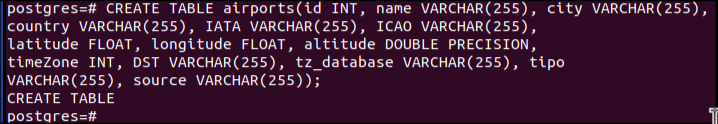
\includegraphics[width=0.8\textwidth]{figures/47.png}
    \caption{Creando la tabla airports en Postgres}
    \label{fig:create_airports_table}
\end{figure}

También deberemos darle una contraseña al usuario \texttt{postgres}:

\begin{lstlisting}[language=sql]
ALTER USER postgres WITH PASSWORD 'postgres';
\end{lstlisting}

\begin{figure}[H]
    \centering
    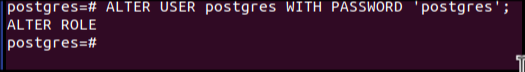
\includegraphics[width=0.8\textwidth]{figures/48.png}
    \caption{Dando una contraseña al usuario postgres}
    \label{fig:postgres_password}
\end{figure}

Guardamos los datos en la tabla \texttt{airports} de Postgres:

\begin{lstlisting}[language=scala]
import java.util.Properties
val properties = new Properties()

properties.setProperty("user", "postgres")
properties.setProperty("driver", "org.postgresql.Driver")
properties.setProperty("password", "postgres")
properties.setProperty("partitionColumn", "altitude")
properties.setProperty("lowerBound", "0")
properties.setProperty("upperBound", "2000")
properties.setProperty("numPartitions", "10")
properties.setProperty("password", "postgres")

df_airports.write.mode("overwrite").jdbc("jdbc:postgresql://localhost:5432/postgres", "airports", properties)
\end{lstlisting}

\begin{figure}[H]
    \centering
    \includegraphics[width=0.8\textwidth]{figures/49.png}
    \caption{Guardando los datos en la tabla airports de Postgres}
    \label{fig:save_airports_postgres}
\end{figure}

Mostramos las 5 filas de la tabla \texttt{airports} de Postgres añadiendo los parámetros necesarios. Los parámetros \texttt{lowerBound} y \texttt{upperBound} se utilizan para definir el rango de valores de la columna \texttt{altitude} y \texttt{numPartitions} para definir el número de particiones. El parámetro \texttt{partitionColumn} se utiliza para definir la columna por la que se particionarán los datos. Es importante utilizar estos parámetros para mejorar el rendimiento de la lectura de los datos.

\begin{lstlisting}[language=scala]
spark.read.option("partitionColumn", "altitude").option("lowerBound", 0).option("upperBound", 2000).option("numPartitions", 10).jdbc("jdbc:postgresql://localhost:5432/postgres", "airports", properties).limit(5).show()
\end{lstlisting}

\begin{figure}[H]
    \centering
    \includegraphics[width=0.8\textwidth]{figures/50.png}
    \caption{5 filas de la tabla airports de Postgres}
    \label{fig:airports_postgres_data}
\end{figure}

\section{Routes}

Antes de comenzar, es necesario utilizar un comando diferente para levantar la shell de spark. El JAR del conector de Cassandra no funciona correctamente, por lo que habrá que cargarlo mediante el paquete:

\begin{lstlisting}[language=bash]
bin/spark-shell --master spark://bigdatapc:7077 --executor-memory 2g --executor-cores 2 --jars jars/postgresql-42.7.3.jar  --packages com.datastax.spark:spark-cassandra-connector_2.12:3.3.0 --conf spark.cassandra.connection.host=localhost
\end{lstlisting}

Los datos sobre rutas (fichero \texttt{routes.dat}) están en formato CSV. Por tanto, estos datos se pueden cargar en un Dataframe con el conector correspondiente y las opciones que se requieran. Una vez obtenido este Dataframe, se debe utilizar el conector de Cassandra para guardar los datos en la tabla \texttt{routes} del keyspace practica.

Creamos el esquema de los datos de las rutas:

\begin{lstlisting}[language=scala]
val routes_schema = StructType(Array(StructField("airline", StringType, true), StructField("airline_id", IntegerType, true), StructField("source_airport", StringType, true), StructField("source_airport_id", IntegerType, true), StructField("destination_airport", StringType, true),StructField("destination_airport_id", IntegerType, true), StructField("codeshare", StringType, true), StructField("stops", IntegerType, true), StructField("equipment", StringType, true)))
\end{lstlisting}

\begin{figure}[H]
    \centering
    \includegraphics[width=0.8\textwidth]{figures/51.png}
    \caption{Creando el esquema de los datos de las rutas}
    \label{fig:create_routes_schema}
\end{figure}

Cargamos los datos en un DataFrame utilizando el esquema creado:

\begin{lstlisting}[language=scala]
val df_routes = spark.read.format("csv").option("header", "false").schema(routes_schema).load("/home/bigdata/practica/routes.dat")
\end{lstlisting}

\begin{figure}[H]
    \centering
    \includegraphics[width=0.8\textwidth]{figures/52.png}
    \caption{Dataframe de las rutas}
    \label{fig:routes_df}
\end{figure}

Vamos a añadir una columna \texttt{route_id} que será la primary key de la tabla \texttt{routes} de Cassandra. Para ello a cada fila le añadiremos un identificador único:

\begin{lstlisting}[language=scala]
import org.apache.spark.sql.functions.monotonically_increasing_id
df_routes = df_routes.withColumn("route_id", monotonically_increasing_id())
\end{lstlisting}

Reordenamos para que la columna \texttt{route_id} sea la primera:

\begin{lstlisting}[language=scala]
df_routes = df_routes.select("route_id", "airline", "airline_id", "source_airport", "source_airport_id", "destination_airport", "destination_airport_id", "codeshare", "stops", "equipment")
\end{lstlisting}

\begin{figure}[H]
    \centering
    \includegraphics[width=0.8\textwidth]{figures/53.png}
    \caption{Dataframe de las rutas con la columna route\_id}
    \label{fig:routes_df_route_id}
\end{figure}

Creamos una nueva terminal y ejecutamos el siguiente comando para contectarnos a la shell de Cassandra:

\begin{lstlisting}[language=bash]
~/apache-cassandra-3.11.16/bin/cqlsh
\end{lstlisting}

\begin{figure}[H]
    \centering
    \includegraphics[width=0.8\textwidth]{figures/54.png}
    \caption{Entrando en la shell de Cassandra}
    \label{fig:enter_cassandra_shell}
\end{figure}

Creamos la tabla \texttt{routes} en el keyspace \texttt{practica}:

\begin{lstlisting}[language=sql]
USE practica;

CREATE TABLE routes (
    route_id int,
    airline text,
    airline_id int,
    source_airport text,
    source_airport_id int,
    destination_airport text,
    destination_airport_id int,
    codeshare text,
    stops int,
    equipment text,
    PRIMARY KEY (route_id)
);
\end{lstlisting}

\begin{figure}[H]
    \centering
    \includegraphics[width=0.8\textwidth]{figures/55.png}
    \caption{Creando la tabla routes en Cassandra}
    \label{fig:create_routes_table}
\end{figure}

Ahora ya podemos guardar los datos en la tabla \texttt{routes} del keyspace \texttt{practica} de Cassandra:

\begin{lstlisting}[language=scala]
df_routes.write.format("org.apache.spark.sql.cassandra").option("spark.cassandra.connection.host", "127.0.0.1").option("spark.cassandra.connection.port", "9042").option("keyspace", "practica").option("table", "routes").option("ttl", "1000").mode("append").save()
\end{lstlisting}

\begin{figure}[H]
    \centering
    \includegraphics[width=0.8\textwidth]{figures/56.png}
    \caption{Guardando los datos en la tabla routes de Cassandra}
    \label{fig:save_routes_cassandra}
\end{figure}

Por último, mostraremos 5 filas de los datos en spark, almacenados en Cassandra:

\begin{lstlisting}[language=sql]
spark.read.format("org.apache.spark.sql.cassandra").option("spark.cassandra.connection.host", "127.0.0.1").option("spark.cassandra.connection.port", "9042").option("keyspace", "practica").option("table", "routes").load().limit(5).show()
\end{lstlisting}

\begin{figure}[H]
    \centering
    \includegraphics[width=0.8\textwidth]{figures/57.png}
    \caption{5 filas de los datos en la tabla routes de Cassandra}
    \label{fig:routes_cassandra_data}
\end{figure}

\chapter{Análisis de datos ingestados en el lago de datos}

En este apartado, se busca realizar una serie de consultas analíticas para demostrar al cliente cómo poder extraer información relevante para su caso de uso. Además, también se busca demostrar cómo persistir datos agregados en una nueva tabla para poder ser consultados de manera más rápida por herramientas de BI o de Dashboarding.

\section{Consultas}

\subsection{Preparación de las consultas}

Para poder ejecutar las consultas vamos a cargar los dataframes que hemos guardado en el lago de datos:

\begin{lstlisting}[language=scala]
import java.util.Properties
val properties = new Properties()

properties.setProperty("user", "postgres")
properties.setProperty("driver", "org.postgresql.Driver")
properties.setProperty("password", "postgres")
properties.setProperty("partitionColumn", "altitude")
properties.setProperty("lowerBound", "0")
properties.setProperty("upperBound", "2000")
properties.setProperty("numPartitions", "10")
properties.setProperty("password", "postgres")

val df_airports = spark.read.option("partitionColumn", "altitude").option("lowerBound", 0).option("upperBound", 2000).option("numPartitions", 10).jdbc("jdbc:postgresql://localhost:5432/postgres", "airports", properties)

val df_airlines = spark.read.format("parquet").load("hdfs://localhost:9000/practica/airlines/")
val df_countries = spark.read.format("csv").option("header", "true").option("inferSchema", "true").load("hdfs://localhost:9000/practica/countries/")

val df_routes=spark.read.format("org.apache.spark.sql.cassandra").option("spark.cassandra.connection.host","127.0.0.1").option("spark.cassandra.connection.port","9042").option("keyspace", "practica").option("table", "routes").load()
\end{lstlisting}

Ahora pasaremos los dataframes a \texttt{TempViews} para poder realizar consultas SQL sobre ellos:

\begin{lstlisting}[language=scala]
df_airports.createOrReplaceTempView("airports")
df_airlines.createOrReplaceTempView("airlines")
df_countries.createOrReplaceTempView("countries")
df_routes.createOrReplaceTempView("routes")
\end{lstlisting}

\begin{figure}[H]
    \centering
    \includegraphics[width=0.8\textwidth]{figures/59.png}
    \caption{Creación de las vistas temporales de los dataframes}
    \label{fig:tempviews}
\end{figure}

\subsection{Consulta 1}

La primera consulta que se nos pide es obtener los aeropuertos con mayor altitud. Para ello, se ha realizado la siguiente consulta:

\begin{lstlisting}[language=scala]
spark.sql("SELECT * FROM airports ORDER BY altitude DESC LIMIT 1").show()
\end{lstlisting}

\begin{figure}[H]
    \centering
    \includegraphics[width=0.8\textwidth]{figures/60.png}
    \caption{Resultado de la consulta de aeropuertos con mayor altitud}
    \label{fig:consulta1}
\end{figure}

\subsection{Consulta 2}

La segunda consulta que se nos pide es obtener el número de aeropuertos que hay en España. Para ello, se ha realizado la siguiente consulta:

\begin{lstlisting}[language=scala]
spark.sql("SELECT COUNT(country) AS airport_count FROM airports WHERE country == 'Spain'").show()
\end{lstlisting}

\begin{figure}[H]
    \centering
    \includegraphics[width=0.8\textwidth]{figures/61.png}
    \caption{Resultado de la consulta de aeropuertos en España}
    \label{fig:consulta2}
\end{figure}

\subsection{Consulta 3}

La tercera consulta que se nos pide es obtener los países que tienen aeropuertos cuyo horario de verano sea el de Europa. Para ello, se ha realizado la siguiente consulta:

\begin{lstlisting}[language=scala]
spark.sql("SELECT DISTINCT country FROM airports WHERE dst == 'E'").show()
\end{lstlisting}

\begin{figure}[H]
    \centering
    \includegraphics[width=0.8\textwidth]{figures/62.png}
    \caption{Resultado de la consulta de países con aeropuertos en horario de verano de Europa}
    \label{fig:consulta3}
\end{figure}

\subsection{Consulta 4}

La cuarta consulta que se nos pide es obtener el número de aerolíneas que tiene EEUU. Como habíamos particionado los datos por país, cargaremos los datos de las aerolíneas de EEUU y contaremos el número de filas:

\begin{lstlisting}[language=scala]
val df_airlines_usa = spark.read.format("parquet").option("header","true").option("inferSchema", "true").load("hdfs://localhost:9000/practica/airlines/country=United States")
df_airlines_usa.count()
\end{lstlisting}

\begin{figure}[H]
    \centering
    \includegraphics[width=0.8\textwidth]{figures/69.png}
    \caption{Resultado de la consulta de aerolíneas en EEUU con particionado por país}
    \label{fig:consulta4-1}
\end{figure}

También se puede realizar la consulta directamente con SQL:

\begin{lstlisting}[language=scala]
spark.sql("SELECT COUNT(*) AS airline_count FROM airlines WHERE country == 'United States'").show()
\end{lstlisting}

\begin{figure}[H]
    \centering
    \includegraphics[width=0.8\textwidth]{figures/63.png}
    \caption{Resultado de la consulta de aerolíneas en EEUU}
    \label{fig:consulta4-2}
\end{figure}

\subsection{Consulta 5}

La quinta consulta que se nos pide es obtener los 10 países con más aerolíneas inactivas. Para ello, se ha realizado la siguiente consulta:

\begin{lstlisting}[language=scala]
spark.sql("SELECT country, COUNT(*) AS inactive_airlines FROM airlines WHERE active == 'f' GROUP BY country ORDER BY inactive_airlines DESC LIMIT 10").show()
\end{lstlisting}

\begin{figure}[H]
    \centering
    \includegraphics[width=0.8\textwidth]{figures/64.png}
    \caption{Resultado de la consulta de países con más aerolíneas inactivas}
    \label{fig:consulta5}
\end{figure}

\subsection{Consulta 6}

La sexta y última consulta que se nos pide es obtener los países que tienen aerolíneas en activo y aeropuertos con una latitud mayor a 80. Para ello, se ha realizado la siguiente consulta:

\begin{lstlisting}[language=scala]
spark.sql("SELECT DISTINCT a.country FROM airports a JOIN airlines b ON a.country = b.country WHERE a.latitude > 80 AND b.active == 't'").show()
\end{lstlisting}

\begin{figure}[H]
    \centering
    \includegraphics[width=0.8\textwidth]{figures/65.png}
    \caption{Resultado de la consulta de países con aerolíneas activas y aeropuertos con latitud mayor a 80}
    \label{fig:consulta6}
\end{figure}

\section{Persistencia de datos agregados}

Por último, también queremos mostrar al cliente la capacidad que tiene nuestra plataforma para guardar datos agregados en tablas nuevas para poder realizar informes o consultar datos específicos con menor procesamiento y menor latencia. 

Para ello, se necesita crear una tabla llamada aggregations que guarde sus datos en formato
parquet en la ruta /practica/aggregations/ de HDFS y que responda a la siguiente pregunta:

- ¿Cuántas rutas sin paradas (stops) a destinos con una altitud (altitude) mayor a 200 metros
se hicieron por país (country) con aerolíneas que ya no están activas (active)?

Para ello, se ha realizado la siguiente consulta:

\begin{lstlisting}[language=scala]
val df_aggregations = spark.sql("SELECT a.country, COUNT(*) AS routes_count FROM airports a JOIN routes r ON a.IATA = r.destination_airport JOIN airlines b ON a.country = b.country WHERE r.stops = 0 AND a.altitude > 200 AND b.active = 'f' GROUP BY a.country")
\end{lstlisting}

\begin{figure}[H]
    \centering
    \includegraphics[width=0.8\textwidth]{figures/66.png}
    \caption{Resultado de la consulta de rutas sin paradas a destinos con altitud mayor a 200 metros por país con aerolíneas inactivas}
    \label{fig:consulta7}
\end{figure}

Ahora ya podemos guardar el dataframe en formato parquet en la ruta /practica/aggregations/ de HDFS:

\begin{lstlisting}[language=scala]
df_aggregations.write.format("parquet").save("hdfs://localhost:9000/practica/aggregations/") 
\end{lstlisting}

\begin{figure}[H]
    \centering
    \includegraphics[width=0.8\textwidth]{figures/67.png}
    \caption{Guardado del dataframe en formato parquet en la ruta /practica/aggregations/ de HDFS}
    \label{fig:guardado}
\end{figure}

Ahora ya podemos consultar la tabla de agregaciones:

\begin{lstlisting}[language=scala]
spark.read.format("parquet").load("hdfs://localhost:9000/practica/aggregations/").show()
\end{lstlisting}

\begin{figure}[H]
    \centering
    \includegraphics[width=0.8\textwidth]{figures/68.png}
    \caption{Resultado de la consulta de la tabla de agregaciones}
    \label{fig:carga-consulta}
\end{figure}


\end{document}
